%\part{Konstruktion}
%\chapter{Programmlogik}
%\section{QueryResolution}

\subsection{QueryBuild}

\begin{figure}[htb]
  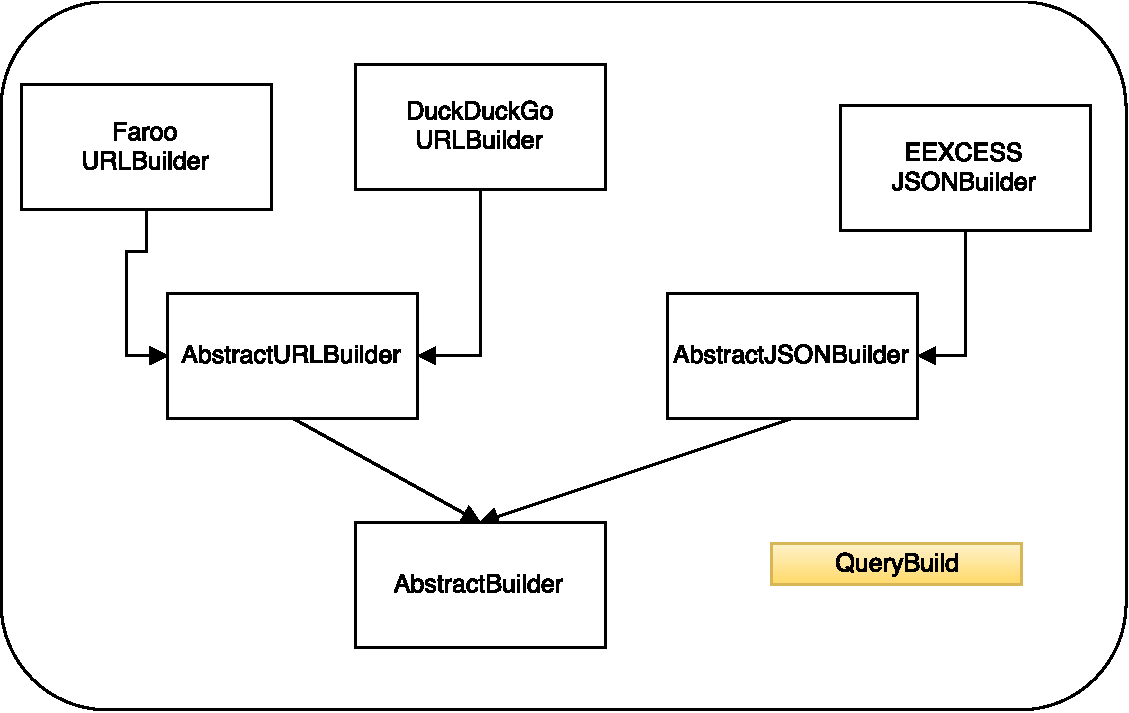
\includegraphics[width=\textwidth]{qr_querybuild}
  \caption{Aufbau des Moduls QueryBuild}
	\label{fig:Aufbau des Moduls QueryBuild}
\end{figure}

Das Modul QueryBuild liefert den größten Teil der Intelligenz im Modul QueryResolution. Die Aufgaben des Moduls sind es, die ConnectionController in QuerySend zu konfigurieren, die Query in das suchmaschinenspezifische Anfrageformat umzuwandeln und dem ConnectionController den Parser für die Antwort zu geben.

Es gibt für jede Suchmaschine eine Implementation der Spezifikation AbstractBuilder, welche durch die Spezifikationen URLAbstractBuilder und JSONAbstractBuilder erweitert wird.

\subsubsection{AbstractBuilder}
\subsubsection{AbstractJSONBuilder}
\subsubsection{AbstractURLBuilder}
\subsubsection{EexcessJSONBuilder}
\subsubsection{FarooURLBuilder}
\subsubsection{DuckDuckGoURLBuilder}
\subsubsection{EEXCESSOrigin}

%\paragraph{Paragraph}
%\subparagraph{Unterparagraph}
